\documentclass{article}
\linespread{1.3}
\usepackage[margin=50pt]{geometry}
\usepackage{amsmath, amsthm, amssymb, amsthm, tikz, fancyhdr}
\pagestyle{fancy}
\renewcommand{\headrulewidth}{0pt}
\newcommand{\changefont}{\fontsize{15}{15}\selectfont}

\fancypagestyle{firstpageheader}
{
  \fancyhead[R]{\changefont Michael Huang \\ CFRM 415 \\ Homework 3}
}

\begin{document}

\thispagestyle{firstpageheader}

\section*{1.}

{\Large 

According to put-call parity, we know that \\
$C - P - S + PV(X) = 0$ \\
$C - P = S - PV(X)$ \\
$C = S - PV(X) + P$ \\
Since $P > 0$, we can see that \\
$C \geq S - PV(X)$ \\
as we aimed to show. \\ \\
% The time value of a call is more the than the time value of a corresponding put.
% Time value part is greater than just share price or loan?
This confirms that the time value is always positive for the European call option, as displayed by the difference between the lines.
% nonnegative?

\begin{figure}[h]
  \centering
  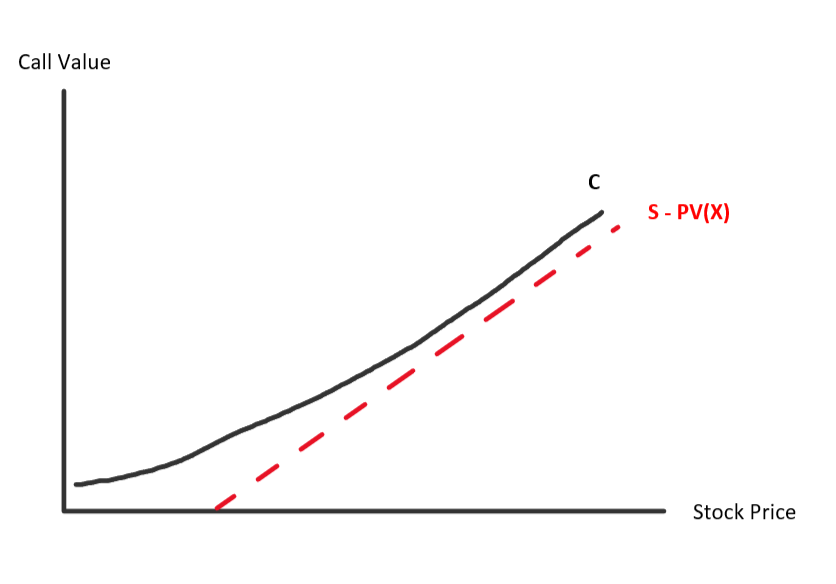
\includegraphics[width=120mm]{./1.png}
\end{figure}

\newpage

}

\section*{2.}
{\Large

\subsection*{(a)}

The trader believes that the stock price $S$ will go below $X$ at time $T$, the time at which they can then exercise the option. 
% Specifically, if the trader pays some premium $P$ on the option, then they would expect the stock price $S$ to go at least $P$ below $X$, or that $S$ will be at most $X - P$ at time $T$. 

\subsection*{(b)}

\begin{figure}[h]
  \centering
  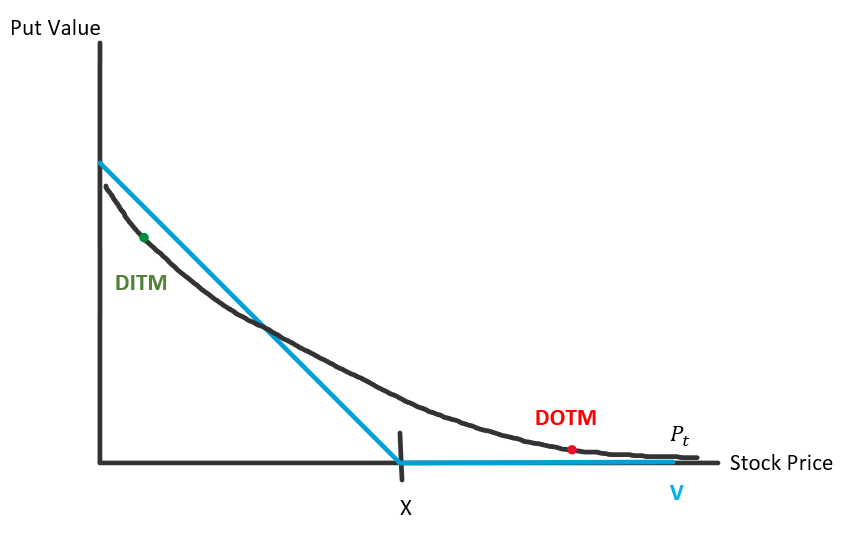
\includegraphics[width=120mm]{./2.png}
\end{figure}

\subsection*{(c)}

See part (b), labeled as $P_t$.

\subsection*{(d)}

See part (b), labeled as $DITM$. \\
The intrinsic value will be relatively high and positive. \\
The time value will be relatively low, and in our case according to the point we picked on the curve, even negative.

\subsection*{(e)}

See part (b), labeled as $DOTM$. \\ \\
The intrinsic value at this point is zero (we cannot exercise the put option for profit, so it is worthless). 
The time value will be higher in comparison with the time value at the point where we are deep in the money. 
% (greater chance of becoming more valuable, depends on t)
% could also be smol, depending on diff between option value at/before expiry

}

\section*{3.}
{\Large 

A European capped call option is like a European call option except that the payoff is $H - X$ for some constant $H > X$, instead of $S - X$, when the terminal stock price exceeds $H$.  Construct a portfolio of European options with an identical payoff. Explain your reasoning. \\ \\

% Relative to the original $(C - P - S + PV(X) = 0)$ 

% identical payoff to $H - X$?
% Buy a European (K, t) call option and sell a European (B + K, t) call option. Determine the payoff of this portfolio at time t. Show that this is equivalent to the payoff at time t of the European (K, t) capped call option. 

% check the notebooks for thoughts

}

\end{document}